\section{Tribler}
\label{sec:Tribler_feat}
Tribler is an application that enables its users to find, consume and share content through a peer-to-peer (P2P) network. The application is currently available for Windows, Mac and Linux. Tribler facilitates finding and sharing content in a fully decentralized way, which means that no central server is needed. Furthermore, to tackle the issue of people who only download(\emph{leech}) content, Tribler makes use of a reputation system which encourages users to actively participate in uploading (\emph{seeding}) content. Tribler also includes a VoD service which allows users to stream videos.

\begin{figure}[h]
	\centering
	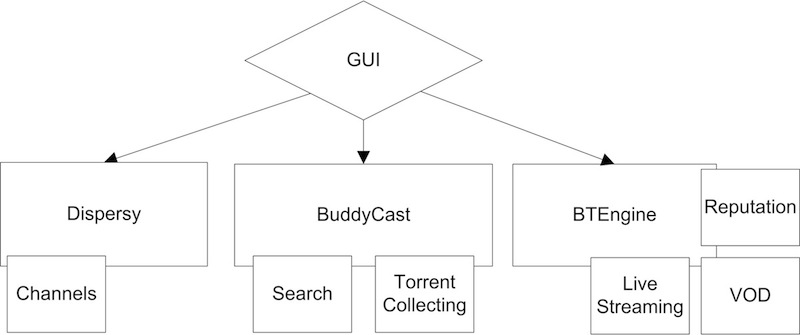
\includegraphics[scale=0.4]{contents/orientation/vod/images/tribler_component_overview.jpg}
	\caption{The architecture of Tribler\protect\footnotemark}
	\label{fig:tribler_components}
\end{figure}
\footnotetext{http://sigmm.org/records/records1201/featured03.html}
\noindent Figure \ref{fig:tribler_components} depicts the four components of Tribler:
\begin{itemize}
	\item GUI: the graphical user interface.
	\item BTengine: An implementation of the BitTorrent protocol.
	\item BuddyCast: a protocol used to find peers with the same taste as the user\cite{tribler}
	\item Dispersy: a fully decentralized system for data bundle synchronization\cite{dispersy}.
\end{itemize}

\subsection{BTengine}
\label{sec:libtorrent_descr}
BitTorrent is a protocol which allows for P2P file sharing. The protocol allows users to join a swarm of hosts to download and upload any file. For a user to share a file it can create a torrent descriptor file which contains information about the file. The torrent can then be distributed over the Internet via e-mail, a link on a website, etc. Other users with the torrent can connect to this host, called a seeder, and ask for pieces of this file. After all pieces are collected, the leecher becomes a seeder and other leechers can download from the new seeder. This way, the files are distributed over the Internet without needing any central server.\\ 
The BTengine in Tribler includes a reputation system, where the user is rated for their upload to download ratio. This helps to minimize the effects of free riding, where users only download, because the user with a low ratio will be given lower speed peers to connect to. As of Tribler 6.1, The BTengine uses an implementation of BitTorrent called: Libtorrent.\\
Libtorrent is a C++ implementation of BitTorrent for embedded devices as well as desktops\footnote{http://www.rasterbar.com/products/libtorrent/}.The interface is well documented and is designed to be CPU- and memory-efficient as well as easy to use.

\subsection{BuddyCast}
The BuddyCast protocol is used to find peers with similar taste, so Tribler can give recommendations to what the user might like and thus discover new content. 

\subsection{Dispersy}
Dispersy is used to spread data bundles over the Internet in a fully decentralized way. This could potentially remove the need for central servers for services such as Facebook or Wikipedia. In Tribler it is used for creating the so called `Channels'. Each channel has different torrents bundled together to form a sort of play list about one topic such a single genre or the new 2013 releases. This makes the discovery of new files that the user might like easier.

\subsection{VoD via P2P} 
\label{sec:download_alg}
By default, pieces of a file are downloaded in a rarity first fashion in the BitTorrent protocol. Tribler implements VoD via P2P by downloading the pieces in the following manner\cite{libswift12}: the download algorithm discerns three priority tiers: high-, middle- and low-priority. The high priority section starts from the current playback position. First it downloads the pieces in this section in-order so that the user experiences continues playback. If no pieces can be downloaded from the high priority section, it will download the pieces in the mid priority section in a rarity first fashion to increase the availability of pieces in the swarm. If the middle priority pieces are also exhausted, it will download the low priority pieces in the same fashion. 

